% ----- Chapter 8 ----- %
%ATS SURVEILLANCE SERVICES %
% Chapter 8 contains procedures applicable by air traffic services units using radar in the performance of their functions.

\chapterbegin

\section[ATS Surveillance Services]{ATS SURVEILLANCE SERVICES}

%References
\note{ADS-contract (ADS-C), at this time used wholly to provide procedural separation, is covered in Chapter 13.}

\subsection[ATS surveillance systems capabilities]{ATS SURVEILLANCE SYSTEMS CAPABILITIES}

\begin{enumnoss}
    \item ATS surveillance systems used in the provision of air traffic services shall have a very high level of reliability, availability and integrity. The possibility of system failures or significant system degradations which may cause complete or partial interruptions of service shall be very remote. Backup facilities shall be provided.
    \note[1]{An ATS surveillance system will normally consist of a number of integrated elements, including sensor(s), data transmission links, data-processing systems and situation displays.}
    \note[2]{Guidance material pertaining to use of radar and to system performance is contained in the \textup{Manual on Testing of Radio Navigation Aids} (Doc 8071), the \textup{Manual on the Secondary Surveillance Radar (SSR) Systems} (Doc 9684) and the \textup{Air Traffic Services Planning Manual} (Doc 9426).}
    \note[3]{Guidance material pertaining to use of ADS-B and MLAT systems and their system performance is contained in Cir 326.}
    \note[4]{Functional and performance requirements pertaining to ATS surveillance systems are contained in \textup{Annex 10} -- Aeronautical Telecommunications, \textup{Volume IV} -- Surveillance and Collision Avoidance Systems.}
    \item ATS surveillance systems should have the capability to receive, process and display, in an integrated manner, data from all the connected sources.
    \item ATS surveillance systems should be capable of integration with other automated systems used in the provision of ATS, and should provide for an appropriate level of automation with the objectives of improving the accuracy and timeliness of data displayed to the controller and reducing controller workload and the need for verbal coordination between adjacent control positions and ATC units.
    \item ATS surveillance systems should provide for the display of safety-related alerts and warnings, including conflict alert, minimum safe altitude warning, conflict prediction and unintentionally duplicated SSR codes and aircraft identification.
    \item States should, to the extent possible, facilitate the sharing of information derived from ATS surveillance systems in order to extend and improve surveillance coverage in adjacent control areas.
    \item States should, on the basis of regional air navigation agreements, provide for the automated exchange of coordination data relevant to aircraft being provided with ATS surveillance services, and establish automated coordination procedures.
    \item ATS surveillance systems, such as primary surveillance radar (PSR), secondary surveillance radar (SSR), ADS-B and MLAT systems may be used either alone or in combination in the provision of air traffic services, including in the provision of separation between aircraft, provided:

    \begin{enumalph}
        \item reliable coverage exists in the area;
        \item the probability of detection, the accuracy and the integrity of the ATS surveillance system(s) are satisfactory; and
        \item in the case of ADS-B, the availability of data from participating aircraft is adequate.
    \end{enumalph}

    \item PSR systems should be used in circumstances where other ATS surveillance systems alone would not meet the air traffic services requirements.
    \item SSR systems, especially those utilizing monopulse techniques or having Mode S capability or MLAT, may be used alone, including in the provision of separation between aircraft, provided:

    \begin{enumalph}
        \item the carriage of SSR transponders is mandatory within the area; and
        \item identification is established and maintained.
    \end{enumalph}

    \item ADS-B shall only be used for the provision of air traffic control service provided the quality of the information contained in the ADS-B message exceeds the values specified by the appropriate ATS authority.
    \item ADS-B may be used alone, including in the provision of separation between aircraft, provided:

    \begin{enumalph}
        \item identification of ADS-B-equipped aircraft is established and maintained;
        \item the data integrity measure in the ADS-B message is adequate to support the separation minimum;
        \item there is no requirement for detection of aircraft not transmitting ADS-B; and
        \item there is no requirement for determination of aircraft position independent of the position-deter\-mining elements of the aircraft navigation system.
    \end{enumalph}

    \item The provision of ATS surveillance services shall be limited to specified areas of coverage and shall be subject to such other limitations as have been specified by the appropriate ATS authority. Adequate information on the operating methods used shall be published in aeronautical information publications, as well as operating practices and/or equipment limitations having direct effects on the operation of the air traffic services.
    %References
    \note{States will provide information on the area or areas where PSR, SSR, ADS-B and MLAT systems are in use as well as ATS surveillance services and procedures in accordance with Annex 15, 4.1.1 and Appendix 1.}

    \begin{enumnoss}
        \item The provision of ATS surveillance services shall be limited when position data quality degrades below a level specified by the appropriate ATS authority.
    \end{enumnoss}

    \item Where PSR and SSR are required to be used in combination, SSR alone may be used in the event of PSR failure to provide separation between identified transponder-equipped aircraft, provided the accuracy of the SSR position indications has been verified by monitor equipment or other means.
\end{enumnoss}

\subsection[Situation display]{SITUATION DISPLAY}

\begin{enumnoss}
    \item A situation display providing surveillance information to the controller shall, as a minimum, include position indications, map information required to provide ATS surveillance services and, where available, information concerning the identity of the aircraft and the aircraft level.
    \item The ATS surveillance system shall provide for a continuously updated presentation of surveillance information, including position indications.
    \item Position indications may be displayed as:

    \begin{enumalph}
        \item individual position symbols, e.g. PSR, SSR, ADS-B or MLAT symbols, or combined symbols;
        \item PSR blips; and
        \item SSR responses.
    \end{enumalph}

    \item When applicable, distinct symbols should be used for presentation of:

    \begin{enumalph}
        \item unintentionally duplicated SSR codes and/or aircraft identification that are unintentionally duplicated;
        \item predicted positions for a non-updated track; and
        \item plot and track data.
    \end{enumalph}

    \item Where surveillance data quality degrades such that services need to be limited, symbology or other means shall be used to provide the controller with an indication of the condition.
    \item Reserved SSR codes, including 7500, 7600 and 7700, operation of IDENT, ADS-B emergency and/or urgency modes, safety-related alerts and warnings as well as information related to automated coordination shall be presented in a clear and distinct manner, providing for ease of recognition.
    \item Labels associated with displayed targets should be used to provide, in alphanumeric form, information derived from the means of surveillance and, where necessary, the flight data processing system.
    \item Labels shall, as a minimum, include information relating to the identity of the aircraft, e.g. SSR code or aircraft identification and, if available, pressure-altitude-derived level information. This information may be obtained from SSR Mode A, SSR Mode C, SSR Mode S and/or ADS-B.
    \item Labels shall be associated with their position indications in a manner precluding erroneous identification by or confusion on the part of the controller. All label information shall be presented in a clear and concise manner.
\end{enumnoss}

\subsection[Communications]{COMMUNICATIONS}

\begin{enumnoss}
    \item The level of reliability and availability of communications systems shall be such that the possibility of system failures or significant degradations is very remote. Adequate backup facilities shall be provided.
    \note{Guidance material and information pertaining to system reliability and availability are contained in Annex 10, Volume I, and the \textup{Air Traffic Services Planning Manual} (Doc 9426).}
    \item Direct pilot-controller communications shall be established prior to the provision of ATS surveillance services, unless special circumstances, such as emergencies, dictate otherwise.
\end{enumnoss}

\subsection[Provision of ATS surveillance services]{PROVISION OF ATS SURVEILLANCE SERVICES}

\begin{enumnoss}
    \item Information derived from ATS surveillance systems, including safety-related alerts and warnings such as conflict alert and minimum safe altitude warning, should be used to the extent possible in the provision of air traffic control service in order to improve capacity and efficiency as well as to enhance safety.
    \item The number of aircraft simultaneously provided with ATS surveillance services shall not exceed that which can safely be handled under the prevailing circumstances, taking into account:

    \begin{enumalph}
        \item the structural complexity of the control area or sector concerned;
        \item the functions to be performed within the control area or sector concerned;
        \item assessments of controller workloads, taking into account different aircraft capabilities, and sector capacity; and
        \item the degree of technical reliability and availability of the primary and backup communications, navigation and surveillance systems, both in the aircraft and on the ground.
    \end{enumalph}
\end{enumnoss}

\subsection[Use of SSR transponders and ADS-B transmitters]{USE OF SSR TRANSPONDERS AND ADS-B TRANSMITTERS}

\subsubsection{General}

To ensure the safe and efficient use of ATS surveillance services, pilots and controllers shall strictly adhere to published operating procedures and standard radiotelephony phraseology shall be used. The correct setting of transponder codes and/or aircraft identification shall be ensured at all times.

\subsubsection{SSR code management}

\begin{enumerate}
    \item Codes 7700, 7600 and 7500 shall be reserved internationally for use by pilots encountering a state of emergency, radiocommunication failure or unlawful interference, respectively.
    \item SSR codes are to be allocated and assigned in accordance with the following principles.
    
    \begin{enumerate}
        \item Codes should be allocated to States or areas in accordance with regional air navigation agreements, taking into account overlapping radar coverage over adjacent airspaces.
        
        %8.5.2.2.2
        \stepcounter{enumii}
        %8.5.2.2.3
        \stepcounter{enumii}

        \item The allocation of a code should preclude the use of this code for any other function within the area of coverage of the same SSR for a prescribed time period.
        \item To reduce pilot and controller workload and the need for controller/pilot communications, the number of code changes required of the pilot should be kept to the minimum.

        %8.5.2.2.6
        \stepcounter{enumii}

        \item Where there is a need for individual aircraft identification, each aircraft shall be assigned a discrete code which should, whenever possible, be retained throughout the flight.
        \item Except for aircraft in a state of emergency, or during communication failure or unlawful interference situations, and unless otherwise agreed by regional air navigation agreement or between a transferring and an accepting ATC unit, the transferring unit shall assign Code A2000 to a controlled flight prior to transfer of communications.
    \end{enumerate}

    % 8.5.2.3
\end{enumerate}

\subsubsection{Operation of SSR transponders}

\note{SSR transponder operating procedures are contained in \textup{Procedures for Air Navigation Services -- Aircraft Operations} (PANS-OPS, Doc 8168), Volume I, Part III, Section 3.}

\begin{enumerate}
    \item When it is observed that the Mode A code shown on the situation display is different to what has been assigned to the aircraft, the pilot shall be requested to confirm the code selected and, if the situation warrants (e.g. not being a case of unlawful interference), to reselect the correct code.
    \item If the discrepancy between assigned and displayed Mode A codes still persists, the pilot may be requested to stop the operation of the aircraft's transponder. The next control position and any other affected unit using SSR and/or MLAT in the provision of ATS shall be informed accordingly.
    \item Aircraft equipped with Mode S having an aircraft identification feature shall transmit the aircraft identification as specified in the flight plan or, when no flight plan has been filed, the aircraft registration.
    \note{All Mode S-equipped aircraft engaged in international civil aviation are required to have an aircraft identification feature (Annex 10, Volume IV, Chapter 2, 2.1.5.2, refers).}
    \item Whenever it is observed on the situation display that the aircraft identification transmitted by a Mode S-equipped aircraft is different from that expected from the aircraft, the pilot shall be requested to confirm and, if necessary, re-enter the correct aircraft identification.
    \item If, following confirmation by the pilot that the correct aircraft identification has been set on the Mode S identification feature, the discrepancy continues to exist, the following actions shall be taken by the controller:

    \begin{enumalph}
        \item inform the pilot of the persistent discrepancy;
        \item where possible, correct the label showing the aircraft identification on the situation display; and
        \item notify the erroneous aircraft identification transmitted by the aircraft to the next control position and any other interested unit using Mode S for identification purposes.
    \end{enumalph}
\end{enumerate}

\subsubsection{Operation of ADS-B transmitters}

\begin{noteev}
    \note[1]{To indicate that it is in a state of emergency or to transmit other urgent information, an aircraft equipped with ADS-B might operate the emergency and/or urgency mode as follows:} \label{8.5.4N1}
    \begin{enumalph}
        \item emergency;
        \item communication failure;
        \item unlawful interference;
        \item minimum fuel; and/or
        \item medical.
    \end{enumalph}
    \note[2]{Some aircraft equipped with first generation ADS-B avionics do not have the capability described in \hyperref[8.5.4N1]{Note 1} above and only have the capability to transmit a general emergency alert regardless of the code selected by the pilot.}
\end{noteev}

\begin{enumerate}
    \item Aircraft equipped with ADS-B having an aircraft identification feature shall transmit the aircraft identification as specified in the flight plan or, when no flight plan has been filed, the aircraft registration.
    \item Whenever it is observed on the situation display that the aircraft identification transmitted by an ADS-B-equipped aircraft is different from that expected from the aircraft, the pilot shall be requested to confirm and, if necessary, re-enter the correct aircraft identification.
    \item If, following confirmation by the pilot that the correct aircraft identification has been set on the ADS-B identification feature, the discrepancy continues to exist, the following actions shall be taken by the controller:

    \begin{enumalph}
        \item inform the pilot of the persistent discrepancy;
        \item where possible, correct the label showing the aircraft identification on the situation display; and
        \item notify the next control position and any other unit concerned of the erroneous aircraft identification transmitted by the aircraft.
    \end{enumalph}
\end{enumerate}

\subsubsection[Level information based on the use of pressure-altitude information]{Level information based on the \\ use of pressure-altitude information}

\begin{enumeratesc}
    \itemsc{Verification of level information}
    \begin{enumerate}
        \item The tolerance value used to determine that pressure-altitude-derived level information displayed to the controller is accurate shall be $\pm$200 ft in RVSM airspace. In other airspace, it shall be $\pm$300 ft, except that the appropriate ATS authority may specify a smaller criterion, but not less than $\pm$200 ft, if this is found to be more practical. Geometric height information shall not be used for separation.
        \item Verification of pressure-altitude-derived level information displayed to the controller shall be effected at least once by each suitably equipped ATC unit on initial contact with the aircraft concerned or, if this is not feasible, as soon as possible thereafter. The verification shall be effected by simultaneous comparison with altimeter-derived level information received from the same aircraft by radiotelephony. The pilot of the aircraft whose pressure-altitude-derived level information is within the approved tolerance value need not be advised of such verification. Geometric height information shall not be used to determine if altitude differences exist.
        \item If the displayed level information is not within the approved tolerance value or when a discrepancy in excess of the approved tolerance value is detected subsequent to verification, the pilot shall be advised accordingly and requested to check the pressure setting and confirm the aircraft's level.
        \item If, following confirmation of the correct pressure setting the discrepancy continues to exist, the following action should be taken according to circumstances:

        \begin{enumalph}
            \item request the pilot to stop Mode C or ADS-B altitude data transmission, provided this does not cause the loss of position and identity information, and notify the next control positions or ATC unit concerned with the aircraft of the action taken; or
            \item inform the pilot of the discrepancy and request that the relevant operation continue in order to prevent loss of position and identity information of the aircraft and, when authorized by the appropriate ATS authority, override the label-displayed level information with the reported level. Notify the next control position or ATC unit concerned with the aircraft of the action taken.
        \end{enumalph}
    \end{enumerate}

    \itemsc{Determination of level occupancy}
    \begin{enumerate}
        \item \label{8.5.5.2.1} The criterion which shall be used to determine that a specific level is occupied by an aircraft shall be $\pm$200 ft in RVSM airspace. In other airspace, it shall be $\pm$300 ft, except that the appropriate ATS authority may specify a smaller criterion, but not less than $\pm$200 ft, if this is found to be more practical.
        \note{For a brief explanation of the considerations underlying this value, see the \textup{Air Traffic Services Planning Manual} (Doc 9426).}
        \item \textit{Aircraft maintaining a level.} An aircraft is considered to be maintaining its assigned level as long as the pressure-altitude-derived level information indicates that it is within the appropriate tolerances of the assigned level, as specified in \ref{8.5.5.2.1}.
        \item \textit{Aircraft vacating a level.} An aircraft cleared to leave a level is considered to have commenced its manoeuvre and vacated the previously occupied level when the pressure-altitude-derived level information indicates a change of more than 300 ft in the anticipated direction from its previously assigned level.
        \item \textit{Aircraft passing a level in climb or descent.} An aircraft in climb or descent is considered to have crossed a level when the pressure-altitude-derived level information indicates that it has passed this level in the required direction by more than 300 ft.
        \item \textit{Aircraft reaching a level.} An aircraft is considered to have reached the level to which it has been cleared when the elapsed time of three display updates, three sensor updates or 15 seconds, whichever is the greater, has passed since the pressure-altitude-derived level information has indicated that it is within the appropriate tolerances of the assigned level, as specified in \ref{8.5.5.2.1}.
        \item Intervention by a controller shall only be required if differences in level information between that displayed to the controller and that used for control purposes are in excess of the values stated above.
    \end{enumerate}
\end{enumeratesc}

\subsection[General procedures]{GENERAL PROCEDURES}

% 8.6.1
\stepcounter{subsubsection}

\subsubsection{Identification of aircraft}

\begin{enumeratesc}
    \itemsc{Establishment of identification}
    \begin{enumerate}
        \item Before providing an ATS surveillance service to an aircraft, identification shall be established and the pilot informed. Thereafter, identification shall be maintained until termination of the ATS surveillance service.
        \item If identification is subsequently lost, the pilot shall be informed accordingly and, when applicable, appropriate instructions issued.
        \item Identification shall be established by at least one of the methods specified in \ref{8.6.2.2}, \ref{8.6.2.3}, \ref{8.6.2.4} and \ref{8.6.2.5}.
    \end{enumerate}

    \itemsc{ADS-B identification procedures} \label{8.6.2.2}
    \begin{enumempty}
        \item Where ADS-B is used for identification, aircraft may be identified by one or more of the following procedures:
    \end{enumempty}
    \begin{enumalph}
        \item direct recognition of the aircraft identification in an ADS-B label;
        \item transfer of ADS-B identification (see \ref{8.6.3}); and
        \item observation of compliance with an instruction to TRANSMIT ADS-B IDENT.
        \note[1]{Some aircraft equipped with first generation ADS-B avionics do not have the capability of squawking IDENT while the emergency and/or urgency mode is selected.}
        \note[2]{In automated systems, the ``IDENT" feature may be presented in different ways, e.g. as a flashing of all or part of the position indication and associated label.}
    \end{enumalph}
    
    \itemsc{SSR and/or MLAT identification procedures} \label{8.6.2.3}
    \begin{enumerate}
        \item Where SSR and/or MLAT is used for identification, aircraft may be identified by one or more of the following procedures:
        
        \begin{enumalph}
            \item recognition of the aircraft identification in an SSR and/or MLAT label;
            \note{The use of this procedure requires that the code/call sign correlation is achieved successfully, taking into account the \hyperref[8.6.2.3.1b]{Note following \ref{8.6.2.3.1b}} below.}
            \item \label{8.6.2.3.1b} recognition of an assigned discrete code, the setting of which has been verified, in an SSR and/or MLAT label;
            %References
            \note{The use of this procedure requires a system of code assignment which ensures that each aircraft in a given portion of airspace is assigned a discrete code (see 8.5.2.2.7).}
            \item direct recognition of the aircraft identification of a Mode S-equipped aircraft in an SSR and/or MLAT label;
            \note{The aircraft identification feature available in Mode S transponders provides the means to identify directly individual aircraft on situation displays and thus offers the potential to eliminate ultimately the recourse to Mode A discrete codes for individual identification. This elimination will only be achieved in a progressive manner depending on the state of deployment of suitable ground and airborne installations.}
            \item by transfer of identification (see \ref{8.6.3});
            \item observation of compliance with an instruction to set a specific code;
            \item observation of compliance with an instruction to squawk IDENT.
            \note[1]{In automated radar systems, the ``IDENT" feature may be presented in different ways, e.g. as a flashing of all or part of the position indication and associated label.}
            \note[2]{Garbling of transponder replies may produce ``IDENT"-type of indications. Nearly simultaneous ``IDENT" transmissions within the same area may give rise to errors in identification.}
        \end{enumalph}
        
        \item When a discrete code has been assigned to an aircraft, a check shall be made at the earliest opportunity to ensure that the code set by the pilot is identical to that assigned for the flight. Only after this check has been made shall the discrete code be used as a basis for identification.
    \end{enumerate}

    \itemsc{PSR identification procedures} \label{8.6.2.4}
    \begin{enumerate}
        \item Where PSR is used for identification, aircraft may be identified by one or more of the following procedures:
        
        \begin{enumalph}
            \item by correlating a particular radar position indication with an aircraft reporting its position over, or as bearing and distance from, a point shown on the situation display, and by ascertaining that the track of the particular radar position is consistent with the aircraft path or reported heading;
            
            \begin{noteev}
                \note[1]{Caution must be exercised when employing this method since a position reported in relation to a point may not coincide precisely with the radar position indication of the aircraft on the situation display. The appropriate ATS authority may, therefore, prescribe additional conditions for the application of this method, e.g.:}
                \begin{enumroman}
                    \item a level or levels above which this method may not be applied in respect of specified navigation aids; or
                    \item a distance from the radar site beyond which this method may not be applied.
                \end{enumroman}
                \note[2]{The term ``a point" refers to a geographical point suitable for the purposes of identification. It is normally a reporting point defined by reference to a radio navigation aid or aids.}
            \end{noteev}
            
            \item by correlating an observed radar position indication with an aircraft which is known to have just departed, provided that the identification is established within 1 NM from the end of the runway used. Particular care should be taken to avoid confusion with aircraft holding over or overflying the aerodrome, or with aircraft departing from or making a missed approach over adjacent runways;
            \item by transfer of identification (see \ref{8.6.3});
            \item by ascertaining the aircraft heading, if circumstances require, and following a period of track observation:
            
            \begin{enumerate}[label=---,labelsep=0.3cm,leftmargin=*,labelindent=0pt]
                \item instructing the pilot to execute one or more changes of heading of 30 degrees or more and correlating the movements of one particular radar position indication with the aircraft's acknowledged execution of the instructions given; or
                \item correlating the movements of a particular radar position indication with manoeuvres currently executed by an aircraft having so reported.
            \end{enumerate}
            
            \noindent When using these methods, the controller shall:
            
            \begin{enumroman}
                \item verify that the movements of not more than one radar position indication correspond with those of the aircraft; and
                \item \label{8.6.2.4.1dii} ensure that the manoeuvre(s) will not carry the aircraft outside the coverage of the radar or the situation display.
            \end{enumroman}
        
            \note[1]{Caution must be exercised when employing these methods in areas where route changes normally take place.}
            \note[2]{With reference to \ref{8.6.2.4.1dii} above, see also \ref{8.6.5.1} regarding vectoring of controlled aircraft.}
        \end{enumalph}
    
        \item Use may be made of direction-finding bearings to assist in identification of an aircraft. This method, however, shall not be used as the sole means of establishing identification, unless so prescribed by the appropriate ATS authority for particular cases under specified conditions.
    \end{enumerate}

    \itemsc{Additional identification method} \label{8.6.2.5}
    \begin{enumempty}
        \item When two or more position indications are observed in close proximity, or are observed to be making similar movements at the same time, or when doubt exists as to the identity of a position indication for any other reason, changes of heading should be prescribed or repeated as many times as necessary, or additional methods of identification should be employed, until all risk of error in identification is eliminated.
    \end{enumempty}    
\end{enumeratesc}

\subsubsection{Transfer of identification} \label{8.6.3}

\begin{enumerate}
    \item Transfer of identification from one controller to another should only be attempted when it is considered that the aircraft is within the accepting controller's surveillance coverage.
    \item Transfer of identification shall be effected by one of the following methods:
    
    \begin{enumalph}
        \item designation of the position indication by automated means, provided that only one position indication is thereby indicated and there is no possible doubt of correct identification;
        \item notification of the aircraft's discrete SSR code or aircraft address;
        %References
        \note[1]{The use of a discrete SSR code requires a system of code assignment which ensures that each aircraft in a given portion of airspace is assigned a discrete code (see 8.5.2.2.7).}
        \note[2]{Aircraft address would be expressed in the form of the alphanumerical code of six hexadecimal characters.}
        \item notification that the aircraft is SSR Mode S-equipped with an aircraft identification feature when SSR Mode S coverage is available;
        \item notification that the aircraft is ADS-B-equipped with an aircraft identification feature when compatible ADS-B coverage is available;
        \item direct designation (pointing with the finger) of the position indication, if the two situation displays are adjacent, or if a common ``conference" type of situation display is used;
        \note{Attention must be given to any errors which might occur due to parallax effects.}
        \item designation of the position indication by reference to, or in terms of bearing and distance from, a geographical position or navigational facility accurately indicated on both situation displays, together with the track of the observed position indication if the route of the aircraft is not known to both controllers;
        
        \begin{noteev}
            \note{Caution must be exercised before transferring identification using this method, particularly if other position indications are observed on similar headings and in close proximity to the aircraft under control. Inherent radar deficiencies, such as inaccuracies in bearing and distance of the radar position indications displayed on individual situation displays and parallax errors, may cause the indicated position of an aircraft in relation to the known point to differ between the two situation displays. The appropriate ATS authority may, therefore, prescribe additional conditions for the application of this method, e.g.:}
            \begin{enumroman}
                \item a maximum distance from the common reference point used by the two controllers; and
                \item a maximum distance between the position indication as observed by the accepting controller and the one stated by the transferring controller.
            \end{enumroman}
        \end{noteev}

        \item \label{8.6.3.2g} where applicable, issuance of an instruction to the aircraft by the transferring controller to change SSR code and the observation of the change by the accepting controller; or
        \item \label{8.6.3.2h} issuance of an instruction to the aircraft by the transferring controller to squawk/transmit IDENT and observation of this response by the accepting controller.
        \note{Use of procedures \ref{8.6.3.2g} and \ref{8.6.3.2h} requires prior coordination between the controllers, since the indications to be observed by the accepting controller are of short duration.}
    \end{enumalph}
\end{enumerate}

\subsubsection{Position information}

\begin{enumerate}
    \item An aircraft provided with ATS surveillance service should be informed of its position in the following circumstances: 
    \begin{enumalph}
        \item upon identification, except when the identification is established:
        
        \begin{enumroman}
            \item based on the pilot's report of the aircraft position or within one nautical mile of the runway upon departure and the observed position on the situation display is consistent with the aircraft's time of departure; or
            \item by use of ADS-B aircraft identification, Mode S aircraft identification or assigned discrete SSR codes and the location of the observed position indication is consistent with the current flight plan of the aircraft; or
            \item by transfer of identification;
        \end{enumroman}

        \item when the pilot requests this information;
        \item when a pilot's estimate differs significantly from the controller's estimate based on the observed position;
        \item when the pilot is instructed to resume own navigation after vectoring if the current instructions had diverted the aircraft from a previously assigned route (see \ref{8.6.5.5});
        \item immediately before termination of ATS surveillance service, if the aircraft is observed to deviate from its intended route.
    \end{enumalph}

    \item \label{8.6.4.2} Position information shall be passed to aircraft in one of the following forms:   
    \begin{enumalph}
        \item as a well-known geographical position;
        \item \label{8.6.4.2b} magnetic track and distance to a significant point, an en-route navigation aid, or an approach aid;
        \item direction (using points of the compass) and distance from a known position;
        \item distance to touchdown, if the aircraft is on final approach; or
        \item distance and direction from the centre line of an ATS route.
    \end{enumalph}

    \item Whenever practicable, position information shall relate to positions or routes pertinent to the navigation of the aircraft concerned and shown on the situation display map.
    \item When so informed, the pilot may omit position reports at compulsory reporting points or report only over those reporting points specified by the air traffic services unit concerned. Unless automated position reporting is in effect (e.g. ADS-C), pilots shall resume voice or CPDLC position reporting:
    
    \begin{enumalph}
        \item when so instructed;
        \item when advised that the ATS surveillance service has been terminated; or
        \item when advised that identification is lost.
    \end{enumalph}
\end{enumerate}

\subsubsection{Vectoring}

\begin{enumerate}
    \item \label{8.6.5.1} Vectoring shall be achieved by issuing to the pilot specific headings which will enable the aircraft to maintain the desired track. When vectoring an aircraft, a controller shall comply with the following:
    
    \begin{enumalph}
        \item whenever practicable, the aircraft shall be vectored along tracks on which the pilot can monitor the aircraft position with reference to pilot-interpreted navigation aids (this will minimize the amount of navigational assistance required and alleviate the consequences resulting from an ATS surveillance system failure);
        \item when an aircraft is given its initial vector diverting it from a previously assigned route, the pilot shall be informed what the vector is to accomplish, and the limit of the vector shall be specified (e.g. to ... position, for ... approach);
        \item except when transfer of control is to be effected, aircraft shall not be vectored closer than 2.5 NM or, where the minimum permissible separation is greater than 5 NM, a distance equivalent to one-half of the prescribed separation minimum, from the limit of the airspace for which the controller is responsible, unless local arrangements have been made to ensure that separation will exist with aircraft operating in adjoining areas;
        \item controlled flights shall not be vectored into uncontrolled airspace except in the case of emergency or in order to circumnavigate adverse meteorological conditions (in which case the pilot should be so informed), or at the specific request of the pilot; and
        \item when an aircraft has reported unreliable directional instruments, the pilot shall be requested, prior to the issuance of manoeuvring instructions, to make all turns at an agreed rate and to carry out the instructions immediately upon receipt.
    \end{enumalph}

    \item When vectoring an IFR flight and when giving an IFR flight a direct routing which takes the aircraft off an ATS route, the controller shall issue clearances such that the prescribed obstacle clearance will exist at all times until the aircraft reaches the point where the pilot will resume own navigation. When necessary, the relevant minimum vectoring altitude shall include a correction for low temperature effect.
    \note[1]{When an IFR flight is being vectored, the pilot may be unable to determine the aircraft's exact position in respect to obstacles in this area and consequently the altitude which provides the required obstacle clearance. Detailed obstacle clearance criteria are contained in PANS-OPS (Doc 8168), Volumes I and II. See also \ref{8.6.8.2}.}
    \note[2]{It is the responsibility of the ATS authority to provide the controller with minimum altitudes corrected for temperature effect.}
    \item Whenever possible, minimum vectoring altitudes should be sufficiently high to minimize activation of aircraft ground proximity warning systems.
    \note{Activation of such systems will induce aircraft to pull up immediately and climb steeply to avoid hazardous terrain, possibly compromising separation between aircraft.}
    
    % 8.6.5.4
    \stepcounter{enumi}

    \item \label{8.6.5.5} In terminating vectoring of an aircraft, the controller shall instruct the pilot to resume own navigation, giving the pilot the aircraft's position and appropriate instructions, as necessary, in the form prescribed in \ref{8.6.4.2} \ref{8.6.4.2b}, if the current instructions had diverted the aircraft from a previously assigned route.
\end{enumerate}

\subsubsection{Navigation assistance}

\begin{enumerate}
    \item An identified aircraft observed to deviate significantly from its intended route or designated holding pattern shall be advised accordingly. Appropriate action shall also be taken if, in the opinion of the controller, such deviation is likely to affect the service being provided.
    \item The pilot of an aircraft requesting navigation assistance from an air traffic control unit providing ATS surveillance services shall state the reason (e.g. to avoid areas of adverse weather or unreliable navigational instruments) and shall give as much information as possible in the circumstances.
\end{enumerate}

\subsubsection{Interruption or termination of ATS surveillance service}

\begin{enumerate}
    \item An aircraft which has been informed that it is provided with ATS surveillance service should be informed immediately when, for any reason, the service is interrupted or terminated.
    \note{The transition of an aircraft across adjoining areas of radar and/or ADS-B and/or MLAT systems coverage will not normally constitute an interruption or termination of the ATS surveillance service.}
    \item When the control of an identified aircraft is to be transferred to a control sector that will provide the aircraft with procedural separation, the transferring controller shall ensure that appropriate procedural separation is established between that aircraft and any other controlled aircraft before the transfer is effected.
\end{enumerate}

\subsubsection{Minimum levels}

\begin{enumerate}
    \item The controller shall at all times be in possession of full and up-to-date information regarding:
    
    \begin{enumalph}
        \item established minimum flight altitudes within the area of responsibility;
        %References
        \item the lowest usable flight level or levels determined in accordance with Chapters \hyperref[4]{4} and 5; and
        \item established minimum altitudes applicable to procedures based on tactical vectoring.
    \end{enumalph}

    \item \label{8.6.8.2} Unless otherwise specified by the appropriate ATS authority, minimum altitudes for procedures based on tactical vectoring with any ATS surveillance system shall be determined using the criteria applicable to tactical radar vectoring.
    \note{Criteria for the determination of minimum altitudes applicable to procedures based on tactical radar
    vectoring are contained in Procedures for \textup{Air Navigation Services -- Aircraft Operations} (PANS-OPS, Doc 8168), Volume II.}
\end{enumerate}

\subsubsection{Information regarding adverse weather}

\begin{enumerate}
    \item Information that an aircraft appears likely to penetrate an area of adverse weather should be issued in sufficient time to permit the pilot to decide on an appropriate course of action, including that of requesting advice on how best to circumnavigate the adverse weather area, if so desired.
    \note{Depending on the capabilities of the ATS surveillance system, areas of adverse weather may not be presented on the situation display. An aircraft's weather radar will normally provide better detection and definition of adverse weather than radar sensors in use by ATS.}
    \item \label{8.6.9.2} In vectoring an aircraft for circumnavigating any area of adverse weather, the controller should ascertain that the aircraft can be returned to its intended or assigned flight path within the coverage of the ATS surveillance system and, if this does not appear possible, inform the pilot of the circumstances.
    \note{Attention must be given to the fact that under certain circumstances the most active area of adverse weather may not be displayed.}
\end{enumerate}

\subsection[Use of ATS surveillance systems in the air traffic control service]{USE OF ATS SURVEILLANCE SYSTEMS IN THE \\ AIR TRAFFIC CONTROL SERVICE}

\note{The procedures in this Section are general procedures applicable when an ATS surveillance system is used in the provision of area control service or approach control service. Additional procedures applicable in the provision of approach control service are detailed in \hyperref[8.9]{Section \ref{8.9}}.}

\subsubsection{Functions}

The information provided by ATS surveillance systems and presented on a situation display may be used to perform the following functions in the provision of air traffic control service:

\begin{enumalph}
    \item provide ATS surveillance services as necessary in order to improve airspace utilization, reduce delays, provide for direct routings and more optimum flight profiles, as well as to enhance safety;
    \item provide vectoring to departing aircraft for the purpose of facilitating an expeditious and efficient departure flow and expediting climb to cruising level;
    \item provide vectoring to aircraft for the purpose of resolving potential conflicts;
    \item provide vectoring to arriving aircraft for the purpose of establishing an expeditious and efficient approach sequence;
    \item provide vectoring to assist pilots in their navigation, e.g. to or from a radio navigation aid, away from or around areas of adverse weather;
    \item provide separation and maintain normal traffic flow when an aircraft experiences communication failure within the area of coverage;
    \item maintain flight path monitoring of air traffic;
    \note{Where tolerances regarding such matters as adherence to track, speed or time have been prescribed by the appropriate ATS authority, deviations are not considered significant until such tolerances are exceeded.}
    \item when applicable, maintain a watch on the progress of air traffic, in order to provide a procedural controller with:
    
    \begin{enumroman}
        \item improved position information regarding aircraft under control;
        \item supplementary information regarding other traffic; and
        \item information regarding any significant deviations by aircraft from the terms of their respective air traffic control clearances, including their cleared routes as well as levels, when appropriate.
    \end{enumroman}
\end{enumalph}

\subsubsection{Separation application}

\note{Factors which the controller using an ATS surveillance system must take into account in determining the spacing to be applied in particular circumstances in order to ensure that the separation minimum is not infringed include aircraft relative headings and speeds, ATS surveillance system technical limitations, controller workload and any difficulties caused by communication congestion. Guidance material on this subject is contained in the \textup{Air Traffic Services Planning Manual} (Doc 9426).}

\begin{enumerate}
    \item Except as provided for in \ref{8.7.2.8}, \ref{8.7.2.9} and \ref{8.8.2.2}, the separation minima specified in \ref{8.7.3} shall only be applied between identified aircraft when there is reasonable assurance that identification will be maintained.
    \item When control of an identified aircraft is to be transferred to a control sector that will provide the aircraft with procedural separation, such separation shall be established by the transferring controller before the aircraft reaches the limits of the transferring controller's area of responsibility, or before the aircraft leaves the relevant area of surveillance coverage.
    \item When authorized by the appropriate ATS authority, separation based on the use of ADS-B, SSR and/or MLAT, and/or PSR position symbols and/or PSR blips shall be applied so that the distance between the centres of the position symbols and/or PSR blips, representing the positions of the aircraft concerned, is never less than a prescribed minimum.
    \item Separation based on the use of PSR blips and SSR responses shall be applied so that the distance between the centre of the PSR blip and the nearest edge of the SSR response (or centre, when authorized by the appropriate ATS authority) is never less than a prescribed minimum.
    \item Separation based on the use of ADS-B position symbols and SSR responses shall be applied so that the distance between the centre of the ADS-B position symbol and the nearest edge of the SSR response (or the centre, when authorized by the appropriate ATS authority) is never less than a prescribed minimum.
    \item Separation based on the use of SSR responses shall be applied so that the distance between the closest edges of the SSR responses (of the centres, when authorized by the appropriate ATS authority) is never less than a prescribed minimum.
    \item In no circumstances shall the edges of the position indications touch or overlap unless vertical separation is applied between the aircraft concerned, irrespective of the type of position indication displayed and separation minimum applied.
    \item \label{8.7.2.8} In the event that the controller has been notified of a controlled flight entering or about to enter the airspace within which the separation minima specified in \ref{8.7.3} is applied, but has not identified the aircraft, the controller may, if so prescribed by the appropriate ATS authority, continue to provide an ATS surveillance service to identified aircraft provided that:
    
    \begin{enumalph}
        \item reasonable assurance exists that the unidentified controlled flight will be identified using SSR and/or ADS-B and/or MLAT or the flight is being operated by an aircraft of a type which may be expected to give an adequate return on primary radar in the airspace within which the separation is applied; and
        \item the separation is maintained between identified flights and any other observed ATS surveillance system position indications until either the unidentified controlled flight has been identified or procedural separation has been established.
    \end{enumalph}

    \item \label{8.7.2.9} The separation minima specified in \ref{8.7.3} may be applied between an aircraft taking off and a preceding departing aircraft or other identified traffic provided there is reasonable assurance that the departing aircraft will be identified within 1 NM from the end of the runway, and that, at the time, the required separation will exist.
    \item The separation minima specified in \ref{8.7.3} shall not be applied between aircraft holding over the same holding fix. Application of ATS surveillance system separation minima based on radar and/or ADS-B and/or MLAT systems between holding aircraft and other flights shall be subject to requirements and procedures prescribed by the appropriate ATS authority.
\end{enumerate}

\subsubsection{Separation minima based on ATS surveillance systems} \label{8.7.3}

\begin{enumerate}
    \item \label{8.7.3.1} Unless otherwise prescribed in accordance with \ref{8.7.3.2}, \ref{8.7.3.3} or \ref{8.7.3.4}, or \ref{6} (with respect to independent and dependent parallel approaches), the horizontal separation minimum based on radar and/or ADS-B and/or MLAT systems shall be 5.0 NM.
    \item \label{8.7.3.2} The separation minimum in \ref{8.7.3.1} may, if so prescribed by the appropriate ATS authority, be reduced, but not below:
    
    \begin{enumalph}
        \item 3.0 NM when radar and/or ADS-B and/or MLAT systems' capabilities at a given location so permit; and
        \item 2.5 NM between succeeding aircraft which are established on the same final approach track within 10 NM of the runway threshold. A reduced separation minimum of 2.5 NM may be applied, provided:
        
        \begin{enumroman}[labelsep=0.1cm]
            \item the average runway occupancy time of landing aircraft is proven, by means such as data collection and statistical analysis and methods based on a theoretical model, not to exceed 50 seconds;
            \item braking action is reported as good and runway occupancy times are not adversely affected by runway contaminants such as slush, snow or ice;
            \item an ATS surveillance system with appropriate azimuth and range resolution and an update rate of 5 seconds or less is used in combination with suitable displays;
            \item the aerodrome controller is able to observe, visually or by means of surface movement radar (SMR), MLAT system or a surface movement guidance and control system (SMGCS), the runway-in-use and associated exit and entry taxiways;
            \item distance-based wake turbulence separation minima in \ref{8.7.3.4}, or as may be prescribed by the appropriate ATS authority (e.g. for specific aircraft types), do not apply;
            \item aircraft approach speeds are closely monitored by the controller and when necessary adjusted so as to ensure that separation is not reduced below the minimum;
            \item aircraft operators and pilots have been made fully aware of the need to exit the runway in an expeditious manner whenever the reduced separation minimum on final approach is applied; and
            \item procedures concerning the application of the reduced minimum are published in AIPs.
        \end{enumroman}
    \end{enumalph}

    \item \label{8.7.3.3} The separation minimum or minima based on radar and/or ADS-B and/or MLAT systems to be applied shall be prescribed by the appropriate ATS authority according to the capability of the particular ATS surveillance system or sensor to accurately identify the aircraft position in relation to the centre of a position symbol, PSR blip, SSR response and taking into account factors which may affect the accuracy of the ATS surveillance system-derived information, such as aircraft range from the radar site and the range scale of the situation display in use.
    \item \label{8.7.3.4} The following distance-based wake turbulence separation minima shall be applied to aircraft being provided with an ATS surveillance service in the approach and departure phases of flight in the circumstances given in \ref{8.7.3.4.1}.

    \begin{tablecenter}{ccc}
        \toprule
        \addlinespace[2mm]
        \multicolumn{2}{c}{\itshape Aircraft category} & \\
        \itshape \makecell{Preceding \\ aircraft} & \itshape \makecell{Succeeding \\ aircraft} & \itshape \makecell{Distance-based \\ wake turbulence \\ separation minima} \\
        \addlinespace[1mm]
        \midrule
        \addlinespace[2mm]
        \multirow{3}{*}{HEAVY} & HEAVY & 4.0 NM \\
        & MEDIUM & 5.0 NM \\
        & LIGHT & 6.0 NM \\
        \addlinespace[3mm]
        MEDIUM & LIGHT & 5.0 NM \\
        \addlinespace[1mm]
        \bottomrule
    \end{tablecenter}      

    \note{The provisions governing wake turbulence aircraft categorization are set forth in \ref{4}, \hyperref[4.9]{Section \ref{4.9}}.}

    \begin{enumerate}
        \item \label{8.7.3.4.1} The minima set out in \ref{8.7.3.4} shall be applied when:     
        \begin{enumalph}
            \item an aircraft is operating directly behind another aircraft at the same altitude or less than 1 000 ft below; or
            \item both aircraft are using the same runway, or parallel runways separated by less than 2 500 ft (760 m); or
            \item an aircraft is crossing behind another aircraft, at the same altitude or less than 1 000 ft below.
        \end{enumalph}

        \note{See Figures \ref{fig:8-1} and \ref{fig:8-2}.}

        %Figures 8-1 8-2
        \vspace{0.5cm}
        \begin{figure}[!ht]
            \centering
            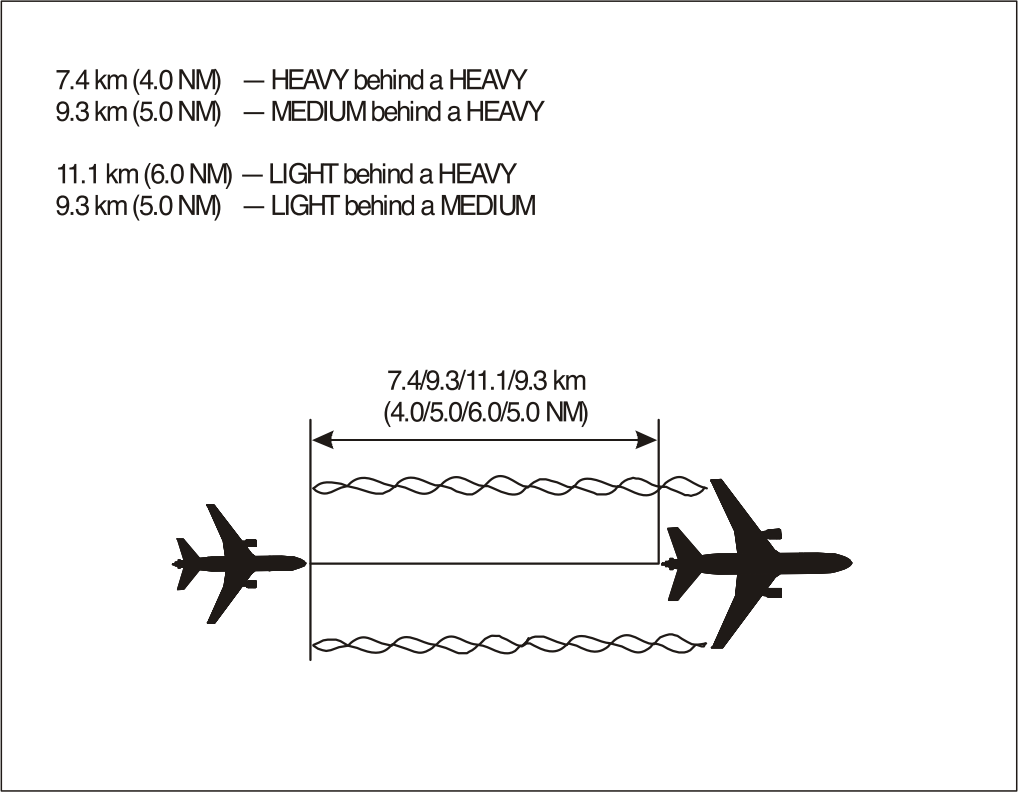
\includegraphics[width=13cm]{Images/Fig 8-1.png}
            \caption[Operating directly behind]{Operating directly behind (see \ref{8.7.3.4} and \ref{8.7.3.4.1})}
            \label{fig:8-1}
        \end{figure}

        \vfill
        \begin{figure}[!ht]
            \centering
            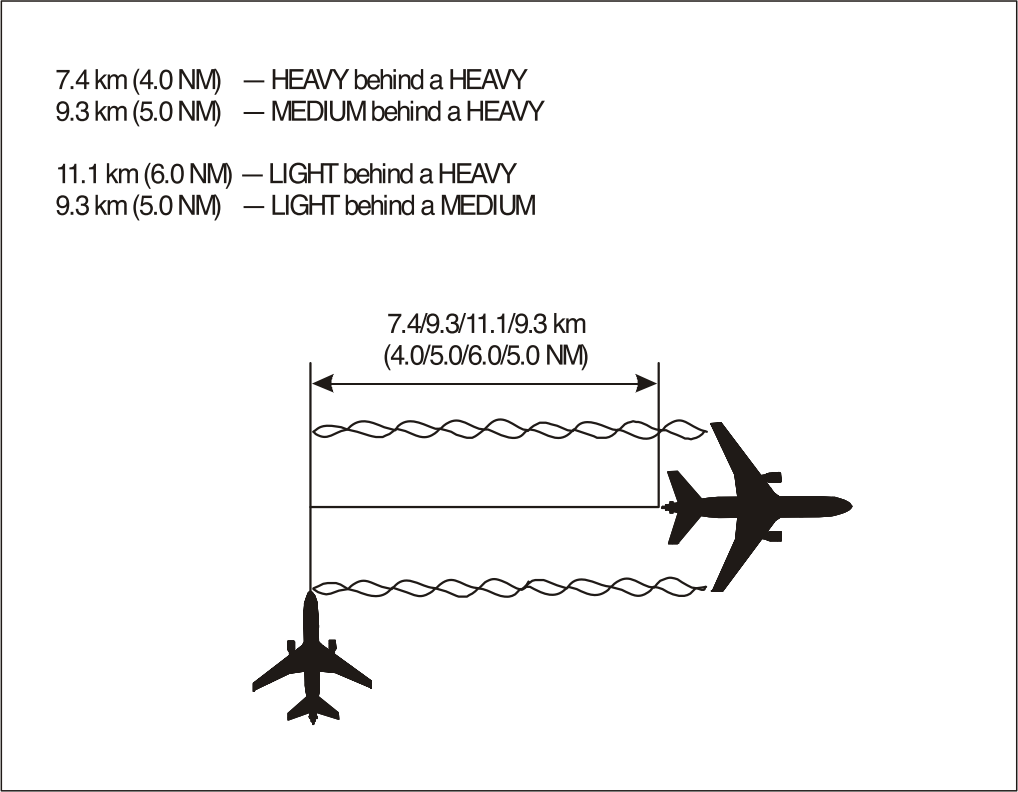
\includegraphics[width=13cm]{Images/Fig 8-2.png}
            \caption[Crossing behind]{Crossing behind (see \ref{8.7.3.4} and \ref{8.7.3.4.1})}
            \label{fig:8-2}
        \end{figure}
    \end{enumerate}
\end{enumerate}

\subsubsection{Transfer of control}

\begin{enumerate}
    \item Where an ATS surveillance service is being provided, transfer of control should be effected, whenever practicable, so as to enable the uninterrupted provision of the ATS surveillance service.
    \item \label{8.7.4.2} Where SSR and/or ADS-B and/or MLAT is used and the display of position indications with associated labels is provided for, transfer of control of aircraft between adjacent control positions or between adjacent ATC units may be effected without prior coordination, provided that:
    
    \begin{enumalph}
        \item updated flight plan information on the aircraft about to be transferred, including the discrete assigned SSR code or, with respect to Mode S and ADS-B, the aircraft identification, is provided to the accepting controller prior to transfer;
        \item the ATS surveillance system coverage provided to the accepting controller is such that the aircraft concerned is presented on the situation display before the transfer is effected and is identified on, but preferably before, receipt of the initial call;
        \item when the controllers are not physically adjacent, two-way direct speech facilities, which permit communications to be established instantaneously, are available between them at all times;
        \note{``Instantaneous" refers to communications which effectively provide for immediate access between controllers.}
        \item \label{8.7.4.2d} the transfer point or points and all other conditions of application, such as direction of flight, specified levels, transfer of communication points, and especially an agreed minimum separation between aircraft, including that applicable to succeeding aircraft on the same route, about to be transferred as observed on the situation display, have been made the subject of specific instructions (for intra-unit transfer) or of a specific letter of agreement between two adjacent ATC units;
        \item \label{8.7.4.2e} the instructions or letter of agreement specify explicitly that the application of this type of transfer of control may be terminated at any time by the accepting controller, normally with an agreed advance notice;
        \item the accepting controller is informed of any level, speed or vectoring instructions given to the aircraft prior to its transfer and which modify its anticipated flight progress at the point of transfer.
    \end{enumalph}

    \item The minimum agreed separation between aircraft about to be transferred (\ref{8.7.4.2} \ref{8.7.4.2d} refers) and the advance notice (\ref{8.7.4.2} \ref{8.7.4.2e} refers) shall be determined taking into account all relevant technical, operational and other circumstances. If circumstances arise in which these agreed conditions can no longer be satisfied, controllers shall revert to the procedure in \ref{8.7.4.4} until the situation is resolved.
    \item \label{8.7.4.4} Where primary radar is being used, and where another type of ATS surveillance system is employed but the provisions of \ref{8.7.4.2} are not applied, the transfer of control of aircraft between adjacent control positions or between two adjacent ATS units may be effected, provided that:

    \begin{enumalph}
        \item identification has been transferred to or has been established directly by the accepting controller;
        \item when the controllers are not physically adjacent, two-way direct-speech facilities between them are at all times available which permit communications to be established instantaneously;
        \item separation from other controlled flights conforms to the minima authorized for use during transfer of control between the sectors or units concerned;
        \item the accepting controller is informed of any level, speed or vectoring instructions applicable to the aircraft at the point of transfer;
        \item radiocommunication with the aircraft is retained by the transferring controller until the accepting controller has agreed to assume responsibility for providing the ATS surveillance service to the aircraft. Thereafter, the aircraft should be instructed to change over to the appropriate channel and from that point is the responsibility of the accepting controller.
    \end{enumalph}
\end{enumerate}

\subsubsection{Speed control}

Subject to conditions specified by the appropriate ATS authority, including consideration of aircraft performance limitations, a controller may, in order to facilitate sequencing or to reduce the need for vectoring, request aircraft to adjust their speed in a specified manner.
\note{Procedures for speed control instructions are contained in \ref{4}, \hyperref[4.6]{Section 4.6}.}

\subsection[Emergencies, hazards and equipment failures]{EMERGENCIES, HAZARDS AND EQUIPMENT FAILURES}

%References
\note{See also Chapter 15.}

\subsubsection{Emergencies}

\begin{enumerate}
    \item In the event of an aircraft in, or appearing to be in, any form of emergency, every assistance shall be provided by the controller, and the procedures prescribed herein may be varied according to the situation.
    \item The progress of an aircraft in emergency shall be monitored and (whenever possible) plotted on the situation display until the aircraft passes out of coverage of the ATS surveillance system, and position information shall be provided to all air traffic services units which may be able to give assistance to the aircraft. Transfer to adjacent sectors shall also be effected when appropriate.
    \note{If the pilot of an aircraft encountering a state of emergency has previously been directed by ATC to select a specific transponder code and/or an ADS-B emergency mode, that code/mode will normally be maintained unless, in special circumstances, the pilot has decided or has been advised otherwise. Where ATC has not requested a code or emergency mode to be set, the pilot will set the transponder to Mode A Code 7700 and/or the appropriate ADS-B emergency mode.}
    \item Whenever a general ADS-B emergency alert is observed on the situation display and there is no other indication of the particular nature of the emergency, the controller shall take the following action:
    
    \begin{enumalph}
        \item attempt to establish communication with the aircraft to verify the nature of the emergency; or
        \item if no response is received from the aircraft, the controller shall attempt to ascertain if the aircraft is able to receive transmissions from the air traffic control unit by requesting it to execute a specified manoeuvre which can be observed on the situation display.
    \end{enumalph}

    \note[1]{Some aircraft equipped with first generation ADS-B avionics have the capability to transmit a general emergency alert only, regardless of the code selected by the pilot.}
    \note[2]{Some aircraft equipped with first generation ADS-B avionics do not have the capability of squawking IDENT while the emergency and/or urgency mode is selected.}
\end{enumerate}

\subsubsection{Collision hazard information}

\begin{enumerate}
    \item When an identified controlled flight is observed to be on a conflicting path with an unknown aircraft deemed to constitute a collision hazard, the pilot of the controlled flight shall, whenever practicable:
    \begin{enumalph}
        \item be informed of the unknown aircraft, and if so requested by the controlled flight or if, in the opinion of the controller, the situation warrants, a course of avoiding action should be suggested; and
        \item be notified when the conflict no longer exists.
    \end{enumalph}

    \item \label{8.8.2.2} When an identified IFR flight operating outside controlled airspace is observed to be on a conflicting path with another aircraft, the pilot should:
    \begin{enumalph}
        \item be informed as to the need for collision avoidance action to be initiated, and if so requested by the pilot or if, in the opinion of the controller, the situation warrants, a course of avoiding action should be suggested; and
        \item be notified when the conflict no longer exists.
    \end{enumalph}

    \item Information regarding traffic on a conflicting path should be given, whenever practicable, in the following form:
    \begin{enumalph}
        \item relative bearing of the conflicting traffic in terms of the 12-hour clock;
        \item distance from the conflicting traffic in nautical miles (or kilometres);
        \item direction in which the conflicting traffic appears to be proceeding;
        \item level and type of aircraft or, if unknown, relative speed of the conflicting traffic, e.g. slow or fast.
    \end{enumalph}

    \item Pressure-altitude-derived level information, even when unverified, should be used in the provision of collision hazard information because such information, particularly if available from an otherwise unknown aircraft (e.g. a VFR flight) and given to the pilot of a known aircraft, could facilitate the location of a collision hazard.
    \item When the pressure-altitude-derived level information has been verified, the information shall be passed to pilots in a clear and unambiguous manner. If the level information has not been verified, the accuracy of the information should be considered uncertain and the pilot shall be informed accordingly.
\end{enumerate}

% 8.8.3
% 8.8.4
% 8.8.5
% 8.8.6

\subsection[Use of ATS surveillance systems in the approach control service]{USE OF ATS SURVEILLANCE SYSTEMS IN THE \\ APPROACH CONTROL SERVICE} \label{8.9}

\subsubsection{General provisions}

\begin{enumerate}
    \item ATS surveillance systems used in the provision of approach control service shall be appropriate to the functions and level of service to be provided.
    \item ATS surveillance systems used to monitor parallel ILS approaches shall meet the requirements for such operations specified in \ref{6}.
\end{enumerate}

\subsubsection{Functions}

The position indications presented on a situation display may be used to perform the following additional functions in the provision of approach control service:

\begin{enumalph}
    \item provide vectoring of arriving traffic on to pilot-interpreted final approach aids;
    \item provide flight path monitoring of parallel ILS approaches and instruct aircraft to take appropriate action in the event of possible or actual penetrations of the no transgression zone (NTZ);
    \note{See \ref{6}, \hyperref[6.7]{Section 6.7}.}
    \item provide vectoring of arriving traffic to a point from which a visual approach can be completed;
    \item provide vectoring of arriving traffic to a point from which a precision radar approach or a surveillance radar approach can be made;
    \item provide flight path monitoring of other pilot-interpreted approaches;
    \item in accordance with prescribed procedures, conduct:
    
    \begin{enumroman}
        \item surveillance radar approaches;
        \item precision radar (PAR) approaches; and
    \end{enumroman}

    \item provide separation between:
    
    \begin{enumroman}
        \item succeeding departing aircraft;
        \item succeeding arriving aircraft; and
        \item a departing aircraft and a succeeding arriving aircraft.
    \end{enumroman}
\end{enumalph}

\subsubsection[General approach control procedures using ATS surveillance systems]{General approach control procedures \\ using ATS surveillance systems}

\begin{enumerate}
    \item The appropriate ATS authority shall establish procedures to ensure that the aerodrome controller is kept informed of the sequence of arriving aircraft, as well as any instructions and restrictions which have been issued to such aircraft in order to maintain separation after transfer of control to the aerodrome controller.
    \item Prior to, or upon commencement of, vectoring for approach, the pilot shall be advised of the type of approach as well as the runway to be used.
    \item The controller shall advise an aircraft being vectored for an instrument approach of its position at least once prior to commencement of final approach.
    \item When giving distance information, the controller shall specify the point or navigation aid to which the information refers.
    \item The initial and intermediate approach phases of an approach executed under the direction of a controller comprise those parts of the approach from the time vectoring is initiated for the purpose of positioning the aircraft for a final approach, until the aircraft is on final approach and:
    
    \begin{enumalph}
        \item established on the final approach path of a pilot-interpreted aid; or
        \item reports that it is able to complete a visual approach; or
        \item ready to commence a surveillance radar approach; or
        \item transferred to the precision radar approach controller.
    \end{enumalph}

    \item Aircraft vectored for final approach should be given a heading or a series of headings calculated to close with the final approach track. The final vector shall enable the aircraft to be established on the final approach track prior to intercepting the specified or nominal glide path of the approach procedure from below, and should provide an intercept angle with the final approach track of 45 degrees or less.
    \note{See \ref{6}, \hyperref[6.7.3.2]{Section \ref{6.7.3.2}}, and \hyperref[6.7.3.2.3]{Section \ref{6.7.3.2.3}} concerning vectoring and level flight requirements of independent parallel approaches, respectively.}
    \item Whenever an aircraft is assigned a vector which will take it through the final approach track, it should be advised accordingly, stating the reason for the vector.
\end{enumerate}

\subsubsection{Vectoring to pilot-interpreted final approach aid}

\begin{enumerate}
    \item An aircraft vectored to intercept a pilot-interpreted final approach aid shall be instructed to report when established on the final approach track. Clearance for the approach should be issued prior to when the aircraft reports established, unless circumstances preclude the issuance of the clearance at such time. Vectoring will normally terminate at the time the aircraft leaves the last assigned heading to intercept the final approach track.
    \item When clearance for the approach is issued, aircraft shall maintain the last assigned level until intercepting the specified or nominal glide path of the approach procedure. If ATC requires an aircraft to intercept the glide path at a level other than a level flight segment depicted on the instrument approach chart, ATC shall instruct the pilot to maintain the particular level until established on the glide path.
    \item The controller shall be responsible for maintaining separation specified in \ref{8.7.3} between succeeding aircraft on the same final approach, except that the responsibility may be transferred to the aerodrome controller in accordance with procedures prescribed by the appropriate ATS authority and provided an ATS surveillance system is available to the aerodrome controller.
    \item Transfer of control of succeeding aircraft on final approach to the aerodrome controller shall be effected in accordance with procedures prescribed by the appropriate ATS authority.
    \item Transfer of communications to the aerodrome controller should be effected at such a point or time that clearance to land or alternative instructions can be issued to the aircraft in a timely manner.
\end{enumerate}

\subsubsection{Vectoring for visual approach}

\note{See also \ref{6}, \hyperref[6.5.3]{Section \ref{6.5.3}}.}

\begin{enumerate}
    \item The controller may initiate vectoring of an aircraft for visual approach provided the reported ceiling is above the minimum altitude applicable to vectoring and meteorological conditions are such that, with reasonable assurance, a visual approach and landing can be completed.
    \item Clearance for visual approach shall be issued only after the pilot has reported the aerodrome or the preceding aircraft in sight, at which time vectoring would normally be terminated.
\end{enumerate}

\subsubsection{Radar approaches}

\begin{enumeratesc}
    \itemsc{General provisions}
    \begin{enumerate}
        \item During the period that a controller is engaged in giving surveillance radar or precision radar approaches, he or she should not be responsible for any duties other than those directly connected with such approaches.
        \item Controllers conducting radar approaches shall be in possession of information regarding the obstacle clearance altitudes/heights established for the types of approach to be conducted.
        \item Prior to commencement of a radar approach, the aircraft shall be informed of:
        
        \begin{enumalph}
            \item the runway to be used;
            \item the applicable obstacle clearance altitude/height;
            \item the angle of the nominal glide path and, if so prescribed by the appropriate ATS authority or requested by the aircraft, the approximate rate of descent to be maintained;
            \note{See the \textup{Air Traffic Services Planning Manual} (Doc 9426) regarding calculation of approximate rates of descent.}
            \item the procedure to be followed in the event of radiocommunication failure, unless the procedure has been published in AIPs.
        \end{enumalph}

        \item When a radar approach cannot be continued due to any circumstance, the aircraft should be immediately informed that a radar approach or continuation thereof is not possible. The approach should be continued if this is possible using non-radar facilities or if the pilot reports that the approach can be completed visually; otherwise an alternative clearance should be given.
        \item Aircraft making a radar approach should be reminded, when on final approach, to check that the wheels are down and locked.
        \item Unless otherwise prescribed by the appropriate ATS authority, the controller conducting the approach should notify the aerodrome controller or, when applicable, the procedural controller when an aircraft making a radar approach is approximately 8 NM from touchdown. If landing clearance is not received at this time, a subsequent notification should be made at approximately 4 NM from touchdown and landing clearance requested.
        \item Clearance to land or any alternative clearance received from the aerodrome controller or, when applicable, the procedural controller should normally be passed to the aircraft before it reaches a distance of 2 NM from touchdown.
        \item \label{8.9.6.1.8} An aircraft making a radar approach should:
        
        \begin{enumalph}
            \item be directed to execute a missed approach in the following circumstances:
            \begin{enumroman}
                \item when the aircraft appears to be dangerously positioned on final approach; or
                \item for reasons involving traffic conflictions; or
                \item if no clearance to land has been received from the procedural controller by the time the aircraft reaches a distance of 2 NM from touchdown or such other distance as has been agreed with the aerodrome control tower; or
                \item on instructions by the aerodrome controller; or
            \end{enumroman}

            \item be advised to consider executing a missed approach in the following circumstances:
            \begin{enumroman}
                \item when the aircraft reaches a position from which it appears that a successful approach cannot be completed; or
                \item if the aircraft is not visible on the situation display for any significant interval during the last 2 NM of the approach; or
                \item if the position or identification of the aircraft is in doubt during any portion of the final approach.
            \end{enumroman}
        \end{enumalph}

        \noindent In all such cases, the reason for the instruction or the advice should be given to the pilot.

        \item Unless otherwise required by exceptional circumstances, radar instructions concerning a missed approach should be in accordance with the prescribed missed approach procedure and should include the level to which the aircraft is to climb and heading instructions to keep the aircraft within the missed approach area during the missed approach procedure.
    \end{enumerate}
\end{enumeratesc}

\subsubsection{Final approach procedures}

\begin{enumeratesc}
    \itemsc{Surveillance radar approach}
    \begin{enumerate}
        \item A final approach using solely surveillance radar should not be carried out if precision approach radar is available, unless meteorological conditions are such as to indicate with reasonable certainty that a surveillance radar approach can be completed successfully.
        \item A surveillance radar approach shall only be performed with equipment suitably sited and a situation display specifically marked to provide information on position relative to the extended centre line of the runway to be used and distance from touchdown, and which is specifically approved for the purpose by the appropriate ATS authority.
        \item When conducting a surveillance radar approach, the controller shall comply with the following:
        
        \begin{enumalph}
            \item at or before the commencement of the final approach, the aircraft shall be informed of the point at which the surveillance radar approach will be terminated;
            \item the aircraft shall be informed when it is approaching the point at which it is computed that descent should begin, and just before reaching that point it shall be informed of the obstacle clearance altitude/height and instructed to descend and check the applicable minima;

            \item azimuth instructions shall be given in accordance with the precision approach technique (see \ref{8.9.7.2.4});
            \item except as provided in \ref{8.9.7.1.4}, distance from touchdown shall normally be passed at every each NM;
            \item pre-computed levels through which the aircraft should be passing to maintain the glide path shall also be transmitted at every NM at the same time as the distance;
            \item the surveillance radar approach shall be terminated:
            
            \begin{enumroman}
                \item at a distance of 2 NM from touchdown, except as provided in \ref{8.9.7.1.4}; or
                \item before the aircraft enters an area of continuous radar clutter; or
                \item when the pilot reports that a visual approach can be effected;
            \end{enumroman}

            \noindent whichever is the earliest.
        \end{enumalph}

        \item \label{8.9.7.1.4} When, as determined by the appropriate ATS authority, the accuracy of the radar equipment permits, surveillance radar approaches may be continued to the threshold of the runway, or to a prescribed point less than 2 NM from touchdown, in which case:
        \begin{enumalph}
            \item distance and level information shall be given at each half NM;
            \item transmission should not be interrupted for intervals of more than five seconds while the aircraft is within a distance of 4 NM from touchdown;
            \item the controller should not be responsible for any duties other than those directly connected with a particular approach.
        \end{enumalph}

        \item Levels through which the aircraft should pass to maintain the required glide path, and the associated distances from touchdown, shall be pre-computed and displayed in such a manner as to be readily available to the controller concerned.
        \note{See the \textup{Air Traffic Services Planning Manual} (Doc 9426) regarding pre-computation of levels.}
    \end{enumerate}

    \itemsc{Precision radar approach}
    \begin{enumerate}[labelindent=0pt,itemsep=0.2cm]
        \itemscit{Duties of precision approach controller}
        \par\noindent During the period the controller is engaged in giving a precision approach, the controller should not be responsible for any duties other than those directly connected with that particular approach.

        \itemscit{Transfer of control}
        \par\noindent Aircraft to be provided with a precision radar approach shall have been transferred to the controller in charge of the precision approach at a distance of not less than 1 NM from the point of interception of the glide path, unless otherwise provided by the appropriate ATS authority.

        \itemscit{Communications}
        \par\noindent When control of the aircraft is assumed by the controller in charge of the precision approach, a communications check shall be made on the channel to be used during the precision approach and the pilot shall be advised that no further acknowledgement of transmission is required. Thereafter, transmission should not be interrupted for intervals of more than five seconds while the aircraft is on final approach.

        \itemscit{Azimuth information and corrections} \label{8.9.7.2.4}
        \begin{enumerate}
            \item The pilot shall be informed at regular intervals of the aircraft's position in relation to the extended centre line of the runway. Heading corrections shall be given as necessary to bring the aircraft back on to the extended centre line.
            \item In the case of azimuth deviations, the pilot should not take corrective action unless specifically instructed to do so.
        \end{enumerate}

        \itemscit{Elevation information and adjustments}
        \begin{enumerate}
            \item The aircraft shall be informed when it is approaching the point of interception of the glide path and, just before intercepting the glide path, it shall be instructed to begin its descent and to check the applicable decision altitude/height. Thereafter, the aircraft shall be informed at regular intervals of its position in relation to the glide path. When no corrections are required, the aircraft should be informed at regular intervals that it is on the glide path. Deviations from the glide path shall be given to the aircraft, together with instructions to adjust the rate of descent if the corrective action taken by the aircraft does not appear to be sufficient. The aircraft shall be informed when it starts to regain the glide path, and immediately before it reaches the glide path.
            \item In the case of deviations from the glide path, the pilot should take corrective action on the basis of the information given by the controller, even though not specifically instructed to do so.
            \item Prior to the aircraft reaching a point 2 NM from touchdown, or a greater distance as necessary for faster aircraft, a certain degree of tolerance should be allowed with regard to deviations from the glide path, and elevation information need not specify the actual number of feet (or metres) above or below the glide path unless it is required to emphasize the rate of change or the extent of the displacement. Thereafter, any deviations from the glide path should be given to the aircraft, preferably in terms of specific distances (feet or metres) above or below the glide path. The use of emphasis in the manner in which the information is transmitted should normally be sufficient to expedite action by the pilot when necessary (e.g. ``STILL 60 feet too low").
            \item Should the elevation element fail during a precision radar approach, the controller shall inform the aircraft immediately. If possible, the controller shall change to a surveillance radar approach, informing the aircraft of the revised obstacle clearance altitude/height. Alternatively, instructions should be given for a missed approach.
        \end{enumerate}

        \itemscit{Distance information}
        \par\noindent The distance from touchdown should be transmitted at intervals of 1 NM until the aircraft reaches a distance of 4 NM from touchdown. Thereafter distance information should be transmitted at more frequent intervals, priority being given, however, to the provision of azimuth and elevation information and guidance.

        \itemscit{Termination of a precision radar approach}
        \par\noindent A precision radar approach is terminated when the aircraft reaches the point at which the glide path intercepts the obstacle clearance altitude/height. Nevertheless, information shall continue to be given until the aircraft is over the threshold, or at such distance therefrom as may be specified by the appropriate ATS authority, taking into account the capability of the equipment concerned. The approach may be monitored to touchdown and information may continue to be provided as necessary at the discretion of the controller in charge of the precision approach in which case the aircraft shall be informed when it is over the threshold.

        \itemscit{Missed approaches}
        \par\noindent When information provided by the elevation element indicates that the aircraft may be initiating a missed approach, the controller shall take the following action:
        \begin{enumalph}
            \item when there is sufficient time to obtain a reply from the pilot (e.g. when the aircraft is more than 4 km (2 NM) from touchdown), the controller shall transmit the aircraft's height above the glide path and ask if the pilot intends to make a missed approach. If this is confirmed by the pilot, the controller shall pass missed approach instructions (see \ref{8.9.6.1.8});
            \item when there is not sufficient time to obtain a reply from the pilot (e.g. when the aircraft is at 4 km (2 NM) or less from touchdown), the precision approach should be continued, emphasizing the aircraft's displacement, and terminated at the normal termination point. If it is apparent from elevation information that the aircraft is making a missed approach, either before or after the normal termination point, the controller shall pass missed approach instructions (see \ref{8.9.6.1.8}).
        \end{enumalph}
    \end{enumerate}
\end{enumeratesc}

\subsection[Use of ATS surveillance systems in the aerodrome control service]{USE OF ATS SURVEILLANCE SYSTEMS IN THE \\ AERODROME CONTROL SERVICE}

\subsubsection{Functions}

\begin{enumerate}
    \item When authorized by and subject to conditions prescribed by the appropriate ATS authority, ATS surveillance systems may be used in the provision of aerodrome control service to perform the following functions:
    
    \begin{enumalph}
        \item flight path monitoring of aircraft on final approach;
        \item flight path monitoring of other aircraft in the vicinity of the aerodrome;
        \item establishing separation specified in \ref{8.7.3} between succeeding departing aircraft; and
        \item providing navigation assistance to VFR flights.
    \end{enumalph}

    \item Special VFR flights shall not be vectored unless special circumstances, such as emergencies, dictate otherwise.
    \item Caution shall be exercised when vectoring VFR flights so as to ensure that the aircraft concerned does not inadvertently enter instrument meteorological conditions.
    \item In prescribing conditions and procedures for the use of ATS surveillance systems in the provision of aerodrome control service, the appropriate ATS authority shall ensure that the availability and use of an ATS surveillance system will not be detrimental to visual observation of aerodrome traffic.
    \note{Control of aerodrome traffic is in the main based on visual observation of the manoeuvring area and the vicinity of the aerodrome by the aerodrome controller.}
\end{enumerate}

\subsubsection{Use of ATS surveillance systems for surface movement control}

\note{Requirements concerning surface movement guidance and control systems (SMGCS) are contained in
Annex 14, Volume I, Chapter 9. Guidance on the use of surface movement radar (SMR) and other advanced functions is contained in the \textup{Manual of Surface Movement Guidance and Control Systems (SMGCS)} (Doc 9476) and in the \textup{Advanced Surface Movement Guidance and Control Systems (A-SMGCS) Manual} (Doc 9830).}

\begin{enumeratesc}
    \itemsc{General provisions}
    \begin{enumerate}
        \item The use of SMR should be related to the operational conditions and requirements of the particular aerodrome (i.e. visibility conditions, traffic density and aerodrome layout).
        \item SMR systems shall to the extent possible enable the detection and display of the movement of all aircraft and vehicles on the manoeuvring area in a clear and unambiguous manner.
        \item Aircraft and vehicle position indications may be displayed in symbolic or non-symbolic form. Where labels are available for display, the capability should be provided for inclusion of aircraft and vehicle identification by manual or automated means.
    \end{enumerate}

    \itemsc{Functions}
    \begin{enumerate}
        \item SMR should be used to augment visual observation of traffic on the manoeuvring area and to provide surveillance of traffic on those parts of the manoeuvring area which cannot be observed visually.
        \item The information displayed on an SMR display may be used to assist in:
        
        \begin{enumalph}
            \item monitoring of aircraft and vehicles on the manoeuvring area for compliance with clearances and instructions;
            \item determining that a runway is clear of traffic prior to a landing or take-off;
            \item providing information on essential local traffic on or near the manoeuvring area;
            \item determining the location of aircraft and vehicles on the manoeuvring area;
            \item providing directional taxi information to aircraft when requested by the pilot or deemed necessary by the controller. Except under special circumstances, e.g. emergencies, such information should not be issued in the form of specific heading instructions; and
            \item providing assistance and advice to emergency vehicles.
        \end{enumalph}
    \end{enumerate}

    \itemsc{Identification of aircraft}
    \begin{enumempty}
        \item Where an ATS surveillance system is used, aircraft may be identified by one or more of the following procedures:
    \end{enumempty}
    \begin{enumalph}
        \item by correlating a particular position indication with:     
        \begin{enumroman}
            \item an aircraft position visually observed by the controller;
            \item an aircraft position reported by the pilot; or
            \item an identified position indication displayed on a situation display;
        \end{enumroman}
        \item by transfer of identification when authorized by the appropriate ATS authority; and
        \item by automated identification procedures when authorized by the appropriate ATS authority.
    \end{enumalph}
\end{enumeratesc}

\subsection[Use of ATS surveillance systems in the flight information service]{USE OF ATS SURVEILLANCE SYSTEMS IN THE \\ FLIGHT INFORMATION SERVICE}

\note{The use of an ATS surveillance system in the provision of flight information service does not relieve the pilot-in-command of an aircraft of any responsibilities, including the final decision regarding any suggested alteration of the flight plan.}

\subsubsection{Functions}

The information presented on a situation display may be used to provide identified aircraft with:
\begin{enumalph}
    \item information regarding any aircraft observed to be on a conflicting path with the identified aircraft and suggestions or advice regarding avoiding action;
    \item information on the position of significant weather and, as practicable, advice to the aircraft on how best to circumnavigate any such areas of adverse weather (see \hyperref[8.6.9.2]{\ref{8.6.9.2}, Note});
    \item information to assist the aircraft in its navigation.
\end{enumalph}

\chapterend